% ============================================================
%  WIRESHARK FOR SCADA ENGINEERS — COMPREHENSIVE STUDY GUIDE
%  Protocol Analysis & Network Forensics for ICS/OT Networks
%  Covers all 10 chapters: Intro through Protocol Lab
% ============================================================
\documentclass[12pt,twoside,openright]{memoir}

% ── Encoding & fonts ─────────────────────────────────────────
\usepackage[T1]{fontenc}
\usepackage[utf8]{inputenc}
\usepackage{lmodern}
\usepackage{microtype}
\usepackage{palatino}
\usepackage[scaled=0.85]{beramono}

% ── Page geometry ────────────────────────────────────────────
\usepackage[
  top=1.25in, bottom=1.25in,
  inner=1.5in, outer=1.0in,
  marginparwidth=0.8in, marginparsep=0.1in
]{geometry}

% ── Colors ───────────────────────────────────────────────────
\usepackage[dvipsnames,svgnames,x11names]{xcolor}
\definecolor{wsnavy}{HTML}{0C4A6E}
\definecolor{wsblue}{HTML}{0284C7}
\definecolor{wscyan}{HTML}{0EA5E9}
\definecolor{wslight}{HTML}{7DD3FC}
\definecolor{wsorange}{HTML}{EA580C}
\definecolor{wsgreen}{HTML}{15803D}
\definecolor{wsred}{HTML}{DC2626}
\definecolor{wsyellow}{HTML}{D97706}
\definecolor{rowlight}{HTML}{F0F9FF}
\definecolor{rowdark}{HTML}{E0F2FE}
\definecolor{codebg}{HTML}{F8FAFC}
\definecolor{frameborder}{HTML}{475569}
\definecolor{covergray}{HTML}{E0F2FE}
\definecolor{warnbg}{HTML}{FFF7ED}
\definecolor{fieldbg}{HTML}{F0FDF4}

% ── Graphics & TikZ ──────────────────────────────────────────
\usepackage{graphicx}
\usepackage{tikz}
\usetikzlibrary{positioning,shapes.geometric,arrows.meta,decorations.pathreplacing,
                matrix,fit,backgrounds,calc,patterns,shadows.blur}
\usepackage{pgfplots}
\pgfplotsset{compat=1.18}

% ── Tables ───────────────────────────────────────────────────
\usepackage{booktabs}
\usepackage{tabularx}
\usepackage{array}
\usepackage{multirow}
\usepackage{colortbl}
\newcolumntype{L}[1]{>{\raggedright\arraybackslash}p{#1}}
\newcolumntype{C}[1]{>{\centering\arraybackslash}p{#1}}
\newcolumntype{R}[1]{>{\raggedleft\arraybackslash}p{#1}}

% ── Callout boxes ─────────────────────────────────────────────
\usepackage[most,listings]{tcolorbox}

\newtcolorbox{keyconcept}[1][]{
  enhanced, breakable,
  colback=wsblue!8, colframe=wsblue, arc=4pt,
  fonttitle=\bfseries\sffamily\color{white}, title={Key Concept},
  attach boxed title to top left={yshift=-2mm, xshift=6mm},
  boxed title style={colback=wsblue, arc=3pt},
  #1
}

\newtcolorbox{warningbox}[1][]{
  enhanced, breakable,
  colback=warnbg, colframe=wsorange, arc=4pt,
  fonttitle=\bfseries\sffamily\color{white}, title={WARNING},
  attach boxed title to top left={yshift=-2mm, xshift=6mm},
  boxed title style={colback=wsorange, arc=3pt},
  #1
}

\newtcolorbox{example}[2][]{
  enhanced, breakable,
  colback=wsgreen!6, colframe=wsgreen, arc=4pt,
  fonttitle=\bfseries\sffamily\color{white}, title={Example: #2},
  attach boxed title to top left={yshift=-2mm, xshift=6mm},
  boxed title style={colback=wsgreen, arc=3pt},
  #1
}

\newtcolorbox{fieldnote}[1][]{
  enhanced, breakable,
  colback=fieldbg, colframe=wsgreen!60!black, arc=4pt,
  fonttitle=\bfseries\sffamily\color{white}, title={Field Note},
  attach boxed title to top left={yshift=-2mm, xshift=6mm},
  boxed title style={colback=wsgreen!70!black, arc=3pt},
  #1
}

\newtcolorbox{quickref}[1][]{
  enhanced, breakable,
  colback=wsyellow!12, colframe=wsyellow!80!black, arc=4pt,
  fonttitle=\bfseries\sffamily, title={Quick Reference},
  attach boxed title to top left={yshift=-2mm, xshift=6mm},
  boxed title style={colback=wsyellow!80!black, arc=3pt},
  #1
}

\newtcolorbox{commonmistakes}[1][]{
  enhanced, breakable,
  colback=wsred!5, colframe=wsred, arc=4pt,
  fonttitle=\bfseries\sffamily\color{white}, title={Common Mistakes},
  attach boxed title to top left={yshift=-2mm, xshift=6mm},
  boxed title style={colback=wsred, arc=3pt},
  #1
}

\newtcolorbox{filterbox}[1][]{
  enhanced, breakable,
  colback=wsnavy!5, colframe=wsnavy, arc=4pt,
  fonttitle=\bfseries\sffamily\color{white}, title={Filter Reference},
  attach boxed title to top left={yshift=-2mm, xshift=6mm},
  boxed title style={colback=wsnavy, arc=3pt},
  #1
}

% ── Code listings ─────────────────────────────────────────────
\usepackage{listings}
\lstdefinestyle{filterstyle}{
  basicstyle=\ttfamily\small\color{wsnavy},
  backgroundcolor=\color{codebg},
  frame=single, framerule=0.5pt, rulecolor=\color{frameborder},
  breaklines=true, keepspaces=true,
  xleftmargin=10pt, xrightmargin=10pt,
  aboveskip=6pt, belowskip=6pt,
  showstringspaces=false,
  keywordstyle=\color{wsblue}\bfseries,
  commentstyle=\color{wsgreen}\itshape,
  stringstyle=\color{wsorange}
}
\lstset{style=filterstyle}

% ── Headers & footers ────────────────────────────────────────
\usepackage{fancyhdr}
\pagestyle{fancy}
\fancyhf{}
\fancyhead[LE]{\small\sffamily\color{wsblue}\leftmark}
\fancyhead[RO]{\small\sffamily\color{wsblue}\rightmark}
\fancyfoot[LE,RO]{\small\sffamily\thepage}
\fancyfoot[CO,CE]{\small\sffamily\color{gray}Wireshark for SCADA Engineers}
\renewcommand{\headrulewidth}{0.4pt}
\renewcommand{\footrulewidth}{0.2pt}

% ── Hyperref ──────────────────────────────────────────────────
\usepackage[
  colorlinks=true,
  linkcolor=wsblue,
  urlcolor=wscyan,
  citecolor=wsgreen,
  pdfauthor={},
  pdftitle={Wireshark for SCADA Engineers},
  pdfsubject={Protocol Analysis for Industrial Control Systems},
  pdfkeywords={Wireshark, SCADA, Modbus, DNP3, OPC UA, ICS, packet capture},
  bookmarks=true, bookmarksnumbered=true
]{hyperref}

% ── Misc ──────────────────────────────────────────────────────
\usepackage{enumitem}
\usepackage{amsmath}
\usepackage{amssymb}
\usepackage{soul}
\usepackage{mdframed}

% ── Memoir chapter style ──────────────────────────────────────
\makechapterstyle{wireshark}{%
  \renewcommand{\chapnamefont}{\normalfont\Large\sffamily\color{wsblue}}
  \renewcommand{\chapnumfont}{\normalfont\fontsize{56}{56}\bfseries\sffamily\color{wsblue!25}}
  \renewcommand{\chaptitlefont}{\normalfont\Huge\bfseries\sffamily\color{wsnavy}}
  \renewcommand{\printchapternum}{%
    \begin{tikzpicture}[remember picture]
      \node[fill=wsblue!10, rounded corners=6pt,
            inner sep=8pt, minimum width=3cm]{%
        \chapnumfont\thechapter};
    \end{tikzpicture}
  }
  \renewcommand{\afterchapternum}{\par\vspace{4pt}}
  \renewcommand{\afterchaptertitle}{%
    \par\vspace{4pt}
    
\begin{tikzpicture}
      \draw[wsblue, line width=2.5pt] (0,0) -- (\textwidth,0);
      \draw[wsorange, line width=1.2pt] (0,-3pt) -- (3cm,-3pt);
    \end{tikzpicture}
    \par\vspace{16pt}
  }
}
\chapterstyle{wireshark}

\setsecheadstyle{\large\bfseries\sffamily\color{wsblue}}
\setsubsecheadstyle{\normalsize\bfseries\sffamily\color{wsnavy}}
\setsubsubsecheadstyle{\normalsize\itshape\sffamily\color{wsnavy}}

% ── Helper macros ─────────────────────────────────────────────
\newcommand{\filter}[1]{\texttt{\color{wsblue}#1}}
\newcommand{\key}[1]{\textbf{#1}}
\newcommand{\hex}[1]{\texttt{0x#1}}
\newcommand{\port}[1]{\texttt{:#1}}

% ============================================================
%  DOCUMENT BEGIN
% ============================================================
\begin{document}

% ── Title page ───────────────────────────────────────────────
\begin{titlingpage}
\pagecolor{wsnavy}
\color{white}
\vspace*{2cm}
\begin{center}
  {\fontsize{11}{13}\sffamily\color{wslight}\MakeUppercase{Industrial Automation Series}}\\[0.8cm]
  {\fontsize{44}{50}\bfseries\sffamily Wireshark}\\[0.3cm]
  {\fontsize{28}{32}\sffamily\color{wscyan!80} for SCADA Engineers}\\[1.5cm]
  
\begin{tikzpicture}
    \draw[wscyan, line width=2pt] (0,0) -- (10cm,0);
    \draw[wsorange, line width=1pt] (0,-4pt) -- (3cm,-4pt);
  \end{tikzpicture}\\[1.5cm]
  {\large\sffamily\color{covergray}
    Protocol capture, display filters, and dissector analysis\\[0.3cm]
    Modbus, DNP3, and OPC UA on the wire\\[0.3cm]
    Security anomaly detection and field forensics
  }\\[2cm]
  
\begin{tikzpicture}
    \node[draw=wscyan, rounded corners=8pt, inner sep=12pt,
          fill=wsblue!40]{
      \large\sffamily\color{white}
      10 Chapters $\cdot$ Filter Reference $\cdot$ Field War Stories $\cdot$ tshark Cheatsheet
    };
  \end{tikzpicture}
  \vfill
  {\small\sffamily\color{gray} For SCADA and Industrial Automation Engineers}
\end{center}
\end{titlingpage}
\pagecolor{white}\color{black}

% ── Front matter ──────────────────────────────────────────────
\frontmatter
\pagestyle{plain}
\tableofcontents*
\clearpage

% ── Main matter ───────────────────────────────────────────────
\mainmatter
\pagestyle{fancy}

% ============================================================
%  CHAPTER 1: INTRODUCTION TO WIRESHARK
% ============================================================
\chapter{Introduction to Wireshark}

\section{What Wireshark Is}

Wireshark is a network protocol analyzer --- a tool that captures raw frames off a network interface, decodes them according to protocol specifications, and presents the result in a form a human can actually read. It was written by Gerald Combs in 1998, originally under the name Ethereal, and renamed in 2006 when Combs left the company that held the trademark. The software is open source, cross-platform, and free. There is no commercial license required to run it on your industrial network.

The stethoscope analogy is exact: a doctor who guesses at a diagnosis without listening to the patient is a liability. An engineer who guesses at a protocol fault without looking at the wire is doing the same thing. Wireshark ends the guessing.

\begin{keyconcept}[title={What Wireshark Actually Does}]
\begin{enumerate}[noitemsep]
  \item \textbf{Captures} raw Ethernet frames (or serial frames via adapter) from a network interface.
  \item \textbf{Decodes} each frame using protocol dissectors --- built-in or custom code that knows the byte layout of a given protocol.
  \item \textbf{Displays} the result in three panes: packet list, packet detail, and raw hex dump.
  \item \textbf{Filters} traffic using either capture filters (BPF syntax, applied before capture) or display filters (Wireshark syntax, applied post-capture).
\end{enumerate}
\end{keyconcept}

\section{History}

Gerald Combs wrote Ethereal in 1998 as a University of Missouri project. The tool grew into the de facto standard for protocol analysis. In 2006, Combs left CACE Technologies (the corporate sponsor) and took the codebase with him. Unable to take the ``Ethereal'' name --- which was trademarked by CACE --- he renamed it Wireshark. The rename happened over a single weekend. Most of the developer community followed him.

The pcap capture library (libpcap on Unix, WinPcap/Npcap on Windows) was developed independently and predates Wireshark. The pcap file format became the universal exchange format for packet captures --- every major security tool reads it without conversion.

\begin{fieldnote}
The Ukraine power grid attack of December 2015 involved ICS protocols leaving forensic evidence in network captures. Investigators reconstructed the entire attack sequence from PCAP files. The attacker used standard protocols --- Modbus, a remote access tool, and VPN traffic --- all of which Wireshark dissects natively. The investigation that took weeks would have been impossible without packet capture infrastructure in place before the attack.
\end{fieldnote}

\section{The Three-Pane Interface}

\subsection{Packet List Pane (Top)}
One row per captured frame. Default columns: frame number, timestamp, source address, destination address, protocol, length, info summary. The Info column is generated by the dissector and often contains the most useful at-a-glance data: ``Modbus/TCP, Function 3, Read Holding Registers, addr=100, count=10.''

\subsection{Packet Detail Pane (Middle)}
The selected frame expanded into a tree of decoded protocol layers. Each layer corresponds to one protocol in the encapsulation stack. A Modbus TCP frame shows: Frame (Ethernet layer) $\to$ Internet Protocol $\to$ Transmission Control Protocol $\to$ Modbus/TCP. Expanding any node reveals individual fields with their decoded values and byte positions.

\subsection{Packet Bytes Pane (Bottom)}
The raw hex dump of the captured frame, with the currently selected field in the detail pane highlighted. This pane is essential for verifying that the dissector is correct and for reading fields that the dissector does not decode.

\begin{keyconcept}[title={Reading the Hex Dump}]
The bytes pane shows two columns: hexadecimal on the left, ASCII on the right. Non-printable bytes appear as dots. When you click a field in the packet detail pane, the corresponding bytes highlight in both columns. This is how you verify: ``the dissector says Function Code = 3, and the raw byte at offset 7 is 0x03. Correct.''
\end{keyconcept}

\section{Wireshark vs.\ tshark vs.\ dumpcap}

Wireshark ships with several executables that are used in different contexts.

\begin{center}
\begin{tabular}{L{2.5cm}L{9cm}}
\toprule
\rowcolor{wsblue!15}
\textbf{Tool} & \textbf{Purpose} \\
\midrule
\texttt{wireshark} & Full GUI. Interactive analysis. \\
\rowcolor{rowlight}
\texttt{tshark} & Command-line version. Scriptable. Use for automated monitoring, alerts, and headless captures. \\
\texttt{dumpcap} & Capture-only. No analysis. Lower overhead. Used by wireshark/tshark as the underlying capture engine. \\
\rowcolor{rowlight}
\texttt{editcap} & Edit or convert PCAP files: split by packet count, trim time ranges, convert formats. \\
\texttt{mergecap} & Merge multiple PCAP files into one. \\
\rowcolor{rowlight}
\texttt{capinfos} & Print summary statistics about a PCAP file. \\
\bottomrule
\end{tabular}
\end{center}

\begin{warningbox}
Running Wireshark as root (or Administrator) to gain capture access is a security risk. The correct approach: on Linux, add your user to the \texttt{wireshark} group (\texttt{sudo usermod -aG wireshark \$USER}) and restart the session. On Windows, Npcap installs a service that handles privileged capture. Wireshark itself should run as a normal user.
\end{warningbox}

\section{Supported Protocols Relevant to SCADA}

Wireshark includes 3,000$+$ protocol dissectors. Of these, approximately 30 matter for industrial automation. The ones you will use most frequently:

\begin{center}
\begin{tabular}{L{3.2cm}L{2.5cm}L{5.5cm}}
\toprule
\rowcolor{wsblue!15}
\textbf{Protocol} & \textbf{Filter Key} & \textbf{Notes} \\
\midrule
Modbus/TCP & \filter{modbus} & Port 502. Full dissector since Wireshark 1.4. \\
\rowcolor{rowlight}
DNP3 & \filter{dnp3} & Over TCP/UDP port 20000. \\
OPC UA Binary & \filter{opcua} & Port 4840. Detects ``OPC.TCP'' magic bytes. \\
\rowcolor{rowlight}
IEC 60870-5-104 & \filter{iec104} & Port 2404. \\
IEC 61850 MMS & \filter{mms} & Port 102 (over COTP). \\
\rowcolor{rowlight}
EtherNet/IP & \filter{enip} & Port 44818 (TCP) / 2222 (UDP). \\
PROFINET & \filter{pn\_rt} & Ethernet-level, EtherType 0x8892. \\
\rowcolor{rowlight}
BACnet/IP & \filter{bacapp} & Port 47808 (UDP). \\
ICCP & \filter{cotp} & Over ISO transport. \\
\rowcolor{rowlight}
Secure Authentication v5 & \filter{dnp3} & Embedded in DNP3 frames. \\
\bottomrule
\end{tabular}
\end{center}

% ============================================================
%  CHAPTER 2: CAPTURE TECHNIQUES
% ============================================================
\chapter{Capture Techniques \& Interfaces}

\section{The Problem With Switched Networks}

On a hub network, every device received every frame. You plugged in a laptop, set the NIC to promiscuous mode, and you saw everything. Modern networks use switches. A switch learns MAC addresses and forwards frames only to the port of the intended destination. Your laptop plugged into a switch port sees only frames addressed to its own MAC address, plus broadcasts and multicasts. You see almost nothing.

For Wireshark to capture traffic between two other devices on a switched network, you need one of three things: a SPAN port, a network tap, or ARP manipulation (not appropriate for production ICS networks).

\begin{keyconcept}[title={Three Ways to Capture on a Switched Network}]
\begin{enumerate}[noitemsep]
  \item \textbf{SPAN port (Switch Port Analyzer):} Configure the switch to copy frames from one or more source ports to a dedicated mirror port. Connect your capture laptop to the mirror port. Works on managed switches. Every major vendor supports it under some name: SPAN (Cisco), Port Mirroring (HP/Aruba/Juniper).
  \item \textbf{Network tap:} A physical device inserted in-line between two devices. Passes traffic normally, but splits the signal and outputs a copy to a capture port. Completely passive --- the tap introduces no latency and cannot be disabled by software. The correct choice for long-term monitoring.
  \item \textbf{ARP poisoning (man-in-the-middle):} Poisons the ARP cache of two devices to route traffic through your capture machine. \textbf{Do not do this on production ICS networks.} ARP poisoning can disrupt normal communications and cause control system faults.
\end{enumerate}
\end{keyconcept}

\section{SPAN Port Configuration}

A SPAN session on a managed switch copies frames from source ports (or VLANs) to a destination port. Key constraints:
\begin{itemize}[noitemsep]
  \item The SPAN destination port receives copies of all frames from the source. It does not participate in normal switching while SPAN is active.
  \item SPAN has no impact on source port traffic if the switch has sufficient backplane bandwidth. On older or lower-end switches, heavy SPAN sessions can affect performance.
  \item Most switches support only one SPAN destination port.
  \item SPAN copies the frame as seen at the source port --- including VLAN tags if configured for that.
\end{itemize}

\begin{example}{Cisco IOS SPAN Configuration}
\begin{lstlisting}
monitor session 1 source interface GigabitEthernet0/1
monitor session 1 destination interface GigabitEthernet0/24
\end{lstlisting}
This mirrors all traffic on Gi0/1 to Gi0/24. Connect Wireshark to Gi0/24.
\end{example}

\section{Network Taps}

A passive optical or copper tap breaks the physical signal path and outputs a copy to monitor ports. The original devices see no change in behavior. Power failure in the tap passes traffic through (failopen). Benefits over SPAN:
\begin{itemize}[noitemsep]
  \item \textbf{100\% copy.} SPAN can drop packets under load. A passive tap does not.
  \item \textbf{Cannot be disabled remotely.} Physical device in the cable path.
  \item \textbf{No software configuration.} No risk of a misconfigured switch command affecting your capture.
\end{itemize}

\marginpar{\footnotesize\sffamily\color{wsnavy}\textit{Field note:} A tap on the PLC-to-HMI link at a water treatment plant ran for 18 months before anyone looked at the data. The capture revealed that the HMI was polling 10$\times$ more frequently than configured --- a client that had been misconfigured during an upgrade and never caught.}

\section{Promiscuous Mode and Monitor Mode}

\textbf{Promiscuous mode} tells the NIC to accept all frames, not just those addressed to its own MAC. In Wireshark, this is the default behavior and is what you want on a SPAN port or tap. Without promiscuous mode, you would only see frames sent to your own MAC address.

\textbf{Monitor mode} applies specifically to Wi-Fi adapters and allows capture of 802.11 management and control frames in addition to data frames. Not relevant for wired ICS captures but occasionally used for wireless SCADA links or WirelessHART.

\section{Capture Interfaces}

When Wireshark starts, it lists all available capture interfaces with a live throughput sparkline for each. Select the interface connected to your SPAN port or tap. On Windows, interfaces are named by GUID; on Linux, by standard names (eth0, ens33, etc.).

\begin{quickref}
\begin{itemize}[noitemsep]
  \item \textbf{Loopback capture:} Linux: \texttt{lo}. Windows: requires Npcap loopback adapter.
  \item \textbf{Any interface:} Linux supports capturing on ``any'' interface (all interfaces simultaneously). Windows does not.
  \item \textbf{Remote capture:} Capture on a remote machine and pipe to local Wireshark via \texttt{rpcapd} or SSH + dumpcap.
  \item \textbf{USB capture:} Requires USBPcap on Windows. Useful for USB-to-serial adapters running Modbus RTU.
\end{itemize}
\end{quickref}

\section{Capture File Management}

For long-duration captures, writing to a single file is impractical. Use a ring buffer: Wireshark writes to a fixed number of files, then overwrites the oldest.

\begin{example}{Ring Buffer Setup}
In Wireshark: Capture $\to$ Options $\to$ Output tab.\\
Check ``Automatically create a new file after'' and set a size limit (e.g., 100 MB).\\
Check ``Use a ring buffer with'' and set file count (e.g., 10 files).\\
Result: maximum 1\,GB of capture storage, always containing the most recent traffic.

Equivalent tshark command:
\begin{lstlisting}
tshark -i eth0 -b filesize:102400 -b files:10 -w /captures/scada.pcap
\end{lstlisting}
\end{example}

\begin{fieldnote}
A $\$15$ Raspberry Pi Zero W running tshark in a ring buffer, placed on a tap at a critical PLC, gives you 24/7 capture capability with zero licensing cost. When an incident occurs, the PCAP is already there. Every OT environment with untapped critical links is running blind.
\end{fieldnote}

\section{pcap vs.\ pcapng Format}

\begin{center}
\begin{tabular}{L{3cm}L{3.5cm}L{4.5cm}}
\toprule
\rowcolor{wsblue!15}
\textbf{Feature} & \textbf{pcap} & \textbf{pcapng} \\
\midrule
Multiple interfaces & No & Yes \\
\rowcolor{rowlight}
Packet comments & No & Yes \\
Interface metadata & No & Yes \\
\rowcolor{rowlight}
Name resolution & No & Yes (embedded) \\
Compatibility & Universal & Wireshark, Zeek, newer tools \\
\rowcolor{rowlight}
File extension & .pcap & .pcapng \\
\bottomrule
\end{tabular}
\end{center}

Use pcapng for new captures. Use pcap when sharing with tools that do not support pcapng. Wireshark reads both. \texttt{editcap} converts between formats.

\begin{commonmistakes}
\begin{itemize}[noitemsep]
  \item Capturing on the wrong interface --- SPAN destination is Gi0/24 but you selected Gi0/1.
  \item Forgetting to enable promiscuous mode before capturing on a SPAN port.
  \item Using ARP poisoning on a live ICS network.
  \item Capturing to a small disk partition --- ring buffer not configured --- capture dies at disk full.
  \item Expecting a passive tap to show traffic in both directions on one port. Passive taps have separate TX and RX monitor ports; you need two capture interfaces or a merge.
\end{itemize}
\end{commonmistakes}

% ============================================================
%  CHAPTER 3: DISPLAY FILTERS
% ============================================================
\chapter{Display \& Capture Filters}

Wireshark has two entirely separate filter systems. They look similar but use different syntax and are applied at different stages.

\section{Capture Filters vs.\ Display Filters}

\begin{center}
\begin{tabular}{L{3cm}L{5.5cm}L{4cm}}
\toprule
\rowcolor{wsblue!15}
\textbf{} & \textbf{Capture Filter} & \textbf{Display Filter} \\
\midrule
When applied & Before capture, in the kernel & After capture, in Wireshark \\
\rowcolor{rowlight}
Syntax & BPF (Berkeley Packet Filter) & Wireshark filter language \\
Packets dropped & Yes --- filtered packets are lost & No --- all packets kept \\
\rowcolor{rowlight}
Performance & Reduces capture file size & No effect on file size \\
Use case & Known traffic only, disk space limited & Interactive analysis \\
\bottomrule
\end{tabular}
\end{center}

\begin{warningbox}
Capture filters drop packets that do not match. If your capture filter is wrong, you lose the traffic you needed. On production ICS captures, capture with \textbf{no filter} (capture everything) and use display filters for analysis. Disk space is cheap; re-capturing an incident is impossible.
\end{warningbox}

\section{Display Filter Syntax}

Display filters use a field-based language. The general form is:

\begin{center}
\texttt{\color{wsblue}protocol.field \color{wsnavy}operator \color{wsorange}value}
\end{center}

\subsection{Comparison Operators}
\begin{center}
\begin{tabular}{C{2cm}C{2cm}L{6cm}}
\toprule
\rowcolor{wsblue!15}
\textbf{Symbol} & \textbf{Word} & \textbf{Example} \\
\midrule
\texttt{==} & \texttt{eq} & \filter{ip.addr == 192.168.1.100} \\
\rowcolor{rowlight}
\texttt{!=} & \texttt{ne} & \filter{tcp.port != 80} \\
\texttt{>} & \texttt{gt} & \filter{frame.len > 1000} \\
\rowcolor{rowlight}
\texttt{<} & \texttt{lt} & \filter{modbus.func\_code < 10} \\
\texttt{>=} & \texttt{ge} & \filter{tcp.port >= 502} \\
\rowcolor{rowlight}
\texttt{contains} & & \filter{dns.qry.name contains "scada"} \\
\texttt{matches} & & Regular expression match \\
\bottomrule
\end{tabular}
\end{center}

\subsection{Logical Operators}
\begin{center}
\begin{tabular}{C{2cm}C{2cm}C{6cm}}
\toprule
\rowcolor{wsblue!15}
\textbf{Symbol} & \textbf{Word} & \textbf{Example} \\
\midrule
\texttt{\&\&} & \texttt{and} & \filter{ip.src == 10.0.0.1 \&\& tcp.port == 502} \\
\rowcolor{rowlight}
\texttt{||} & \texttt{or} & \filter{modbus || dnp3} \\
\texttt{!} & \texttt{not} & \filter{!arp} \\
\rowcolor{rowlight}
\texttt{()} & & \filter{(modbus || dnp3) \&\& ip.src == 10.0.0.1} \\
\bottomrule
\end{tabular}
\end{center}

\section{Essential SCADA Display Filters}

\begin{filterbox}
\begin{center}
\begin{tabular}{L{5.5cm}L{6cm}}
\toprule
\textbf{Goal} & \textbf{Filter} \\
\midrule
All Modbus traffic & \filter{modbus} \\
Modbus write operations & \filter{modbus.func\_code == 6 || modbus.func\_code == 15 || modbus.func\_code == 16} \\
Modbus exceptions & \filter{modbus.exception\_code > 0} \\
DNP3 traffic & \filter{dnp3} \\
OPC UA traffic & \filter{opcua} \\
Traffic to/from PLC & \filter{ip.addr == 192.168.1.10} \\
Specific TCP conversation & \filter{tcp.stream == 4} \\
Large frames (possible scan) & \filter{frame.len > 1400} \\
ARP traffic & \filter{arp} \\
Retransmissions & \filter{tcp.analysis.retransmission} \\
Zero-window events & \filter{tcp.analysis.zero\_window} \\
Broadcast traffic & \filter{eth.dst == ff:ff:ff:ff:ff:ff} \\
\bottomrule
\end{tabular}
\end{center}
\end{filterbox}

\section{BPF Capture Filter Syntax}

Berkeley Packet Filter syntax is used by \texttt{tcpdump}, \texttt{dumpcap}, and most other capture tools. It is different from Wireshark display filter syntax.

\begin{example}{BPF Capture Filters}
\begin{lstlisting}
port 502                    # Modbus TCP
port 20000                  # DNP3
port 4840                   # OPC UA
host 192.168.1.10           # Traffic to/from specific host
not port 22                 # Exclude SSH management traffic
port 502 or port 20000      # Modbus or DNP3
dst host 192.168.1.1        # Only frames TO this host
net 10.0.0.0/8              # Entire subnet
\end{lstlisting}
\end{example}

\section{Following a TCP Stream}

Individual packets show you individual frames. For a complete conversation, right-click any packet in a TCP session and select ``Follow $\to$ TCP Stream.'' Wireshark reassembles and displays the full byte stream of the session, with bytes from each direction color-coded. This is how you read an entire OPC UA session, a sequence of Modbus requests and responses, or a DNP3 data transfer from start to finish.

\begin{keyconcept}[title={Follow TCP Stream vs.\ Individual Packets}]
The Follow TCP Stream view shows the reassembled application-layer data. It does not show TCP handshake, retransmissions, or TCP overhead. For protocol analysis, it is the right view. For TCP troubleshooting (looking at window sizes, retransmissions, and RTT), use the individual packet view with tcp.* filters.
\end{keyconcept}

\section{Colorization Rules}

Wireshark applies color to rows in the packet list based on configurable rules (View $\to$ Coloring Rules). Default rules highlight TCP errors in red, broadcasts in light blue, and so on. Add custom rules for your environment:

\begin{itemize}[noitemsep]
  \item Modbus write commands in yellow: filter \filter{modbus.func\_code >= 5 \&\& modbus.func\_code != 7}
  \item DNP3 unsolicited responses in orange: filter \filter{dnp3.ctl.uns == 1}
  \item OPC UA sessions with no security in red: \filter{opcua.transport.type == 1} (identify ``None'' mode separately)
\end{itemize}

\begin{commonmistakes}
\begin{itemize}[noitemsep]
  \item Using BPF syntax in the display filter bar (turns red and is ignored).
  \item Using display filter syntax in the capture filter dialog (may appear to work but gives wrong results).
  \item Filtering too aggressively at capture time and discarding context frames needed for analysis.
  \item Confusing \filter{ip.addr == x} (matches either source or destination) with \filter{ip.src == x} (source only).
\end{itemize}
\end{commonmistakes}

% ============================================================
%  CHAPTER 4: PROTOCOL DISSECTORS
% ============================================================
\chapter{Protocol Dissectors \& Decode As}

\section{What a Dissector Does}

A protocol dissector is code that knows the byte layout of a specific protocol and translates a raw byte sequence into named fields with decoded values. Without a dissector, Wireshark shows you hex. With a dissector, it shows you ``Modbus/TCP, Transaction ID: 42, Unit ID: 1, Function: Read Holding Registers (3), Starting Address: 100, Quantity: 10.''

Wireshark selects dissectors using port numbers, EtherType values, and pattern matching. A frame arriving on TCP port 502 is handed to the Modbus/TCP dissector. A frame with EtherType 0x8892 is handed to the PROFINET dissector.

\section{Automatic Protocol Detection}

Wireshark's protocol detection is heuristic. For well-known ports, detection is deterministic: port 502 = Modbus/TCP. For protocols that run on non-standard ports, Wireshark may not identify them correctly.

Common ICS scenarios where automatic detection fails:
\begin{itemize}[noitemsep]
  \item Modbus on a non-standard port (vendor custom implementation using port 1502 or 5020).
  \item DNP3 on a port other than 20000 (some vendors use 20001 or custom ports).
  \item OPC UA Binary on a port other than 4840 (common in vendor-specific configurations).
\end{itemize}

\section{Decode As}

When automatic detection fails, use ``Decode As'' (Analyze $\to$ Decode As, or right-click a packet). This forces Wireshark to apply a specific dissector to packets on a given port or in a given TCP stream.

\begin{example}{Force Modbus Dissector on Port 1502}
\begin{enumerate}[noitemsep]
  \item Right-click a frame that should be Modbus but shows as TCP data.
  \item Select ``Decode As.''
  \item In the Current column, select ``Modbus/TCP.''
  \item Click OK. All frames on that port are now decoded as Modbus.
\end{enumerate}
The Decode As setting persists for the session and can be saved to a profile.
\end{example}

\section{Wireshark Profiles}

A Wireshark profile stores your custom settings: coloring rules, column configuration, display filter toolbar shortcuts, Decode As rules, and preferences. Create a profile for each environment type (Modbus plant, DNP3 substation, OPC UA integration) and switch profiles when connecting to different capture sources.

Profiles are stored in your Wireshark personal configuration directory:
\begin{itemize}[noitemsep]
  \item Linux: \texttt{\textasciitilde/.config/wireshark/profiles/}
  \item Windows: \texttt{\%APPDATA\%\textbackslash Wireshark\textbackslash profiles\textbackslash}
\end{itemize}

\section{Custom Lua Dissectors}

Wireshark supports plugins written in Lua. A Lua dissector can decode a proprietary vendor protocol that has no built-in dissector. The Lua API provides access to the same field registration and tree-building infrastructure used by built-in C dissectors.

\begin{example}{Minimal Lua Dissector Skeleton}
\begin{lstlisting}
local proto_vendor = Proto("vendorproto", "Vendor Protocol")
local f_cmd = ProtoField.uint8("vendorproto.cmd", "Command", base.HEX)
proto_vendor.fields = {f_cmd}

function proto_vendor.dissector(buffer, pinfo, tree)
  pinfo.cols.protocol = "VENDOR"
  local subtree = tree:add(proto_vendor, buffer())
  subtree:add(f_cmd, buffer(0, 1))
end

local tcp_table = DissectorTable.get("tcp.port")
tcp_table:add(9999, proto_vendor)
\end{lstlisting}
Place this file in the Wireshark plugins directory and restart.
\end{example}

\section{Statistics Tools}

Wireshark's Statistics menu provides analysis tools beyond the packet list:

\begin{center}
\begin{tabular}{L{4cm}L{8cm}}
\toprule
\rowcolor{wsblue!15}
\textbf{Tool} & \textbf{Use} \\
\midrule
Protocol Hierarchy & Shows percentage of total traffic by protocol. Identify unexpected protocols instantly. \\
\rowcolor{rowlight}
Conversations & Lists all TCP/UDP/IP conversations with packet counts and byte totals. \\
Endpoints & Lists all network endpoints that appear in the capture. \\
\rowcolor{rowlight}
I/O Graph & Plots packet rate or byte rate over time. Visualize polling intervals and traffic bursts. \\
TCP Stream Graph & RTT, window scaling, throughput graphs for a selected TCP connection. \\
\rowcolor{rowlight}
Expert Information & Aggregates Wireshark's automatic anomaly detection notes. \\
Flow Graph & Ladder diagram of a conversation's packet exchange. \\
\bottomrule
\end{tabular}
\end{center}

\begin{fieldnote}
The Protocol Hierarchy (Statistics $\to$ Protocol Hierarchy) is the first thing to run on any new capture. It tells you what is actually on the network in two seconds. On one site visit, this revealed that 34\% of traffic was NetBIOS Name Service --- a Windows file-sharing protocol that had no business touching the control network. The PLC vendor's Windows-based HMI was doing automatic network browsing every 60 seconds.
\end{fieldnote}

% ============================================================
%  CHAPTER 5: MODBUS ANALYSIS
% ============================================================
\chapter{Analyzing Modbus on the Wire}

\section{The Critical Security Reality}

Modbus has no authentication. No encryption. No sequence numbers. No session concept. Any device with IP connectivity to a Modbus slave can send any function code to any register address, and the slave will execute it. Wireshark makes this viscerally real: every Modbus frame in your capture is readable by anyone who can capture the traffic, and any of those frames could have been sent by a malicious device rather than the legitimate master.

\begin{warningbox}
Modbus TCP operates on port 502. The default configuration of most PLCs and field devices accepts connections from any IP address on port 502. There is no username. There is no password. ``Secure'' Modbus requires network segmentation, firewall rules, and protocol-aware inspection --- none of which are in the Modbus specification itself.
\end{warningbox}

\section{Modbus TCP Frame Structure}

Modbus TCP wraps the core Modbus PDU in a 7-byte MBAP header. The full frame:

\begin{center}
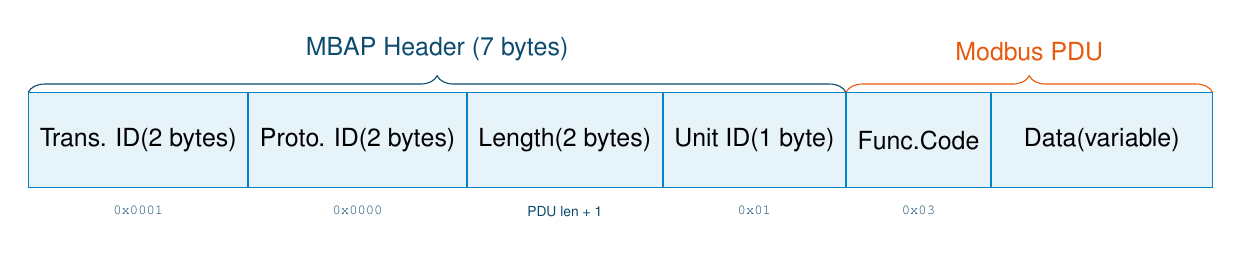
\begin{tikzpicture}[
  box/.style={rectangle, draw=wsblue, fill=wsblue!10, minimum height=1.2cm,
              text centered, font=\small\sffamily, inner sep=4pt},
  label/.style={font=\tiny\sffamily\color{wsnavy}, align=center}
]
\node[box, minimum width=1.8cm] (tid) {Trans. ID\\(2 bytes)};
\node[box, minimum width=1.8cm, right=0pt of tid] (pid) {Proto. ID\\(2 bytes)};
\node[box, minimum width=1.8cm, right=0pt of pid] (len) {Length\\(2 bytes)};
\node[box, minimum width=1.2cm, right=0pt of len] (uid) {Unit ID\\(1 byte)};
\node[box, minimum width=1.2cm, right=0pt of uid] (fc) {Func.\\Code};
\node[box, minimum width=2.8cm, right=0pt of fc] (data) {Data\\(variable)};

\node[label, below=3pt of tid] {\texttt{0x0001}};
\node[label, below=3pt of pid] {\texttt{0x0000}};
\node[label, below=3pt of len] {PDU len + 1};
\node[label, below=3pt of uid] {\texttt{0x01}};
\node[label, below=3pt of fc] {\texttt{0x03}};

\draw [decorate, decoration={brace, amplitude=6pt}, wsnavy]
  (tid.north west) -- (uid.north east) node[midway, above=8pt, font=\small\sffamily\color{wsnavy}]{MBAP Header (7 bytes)};
\draw [decorate, decoration={brace, amplitude=6pt}, wsorange]
  (fc.north west) -- (data.north east) node[midway, above=8pt, font=\small\sffamily\color{wsorange}]{Modbus PDU};
\end{tikzpicture}
\end{center}

\subsection{MBAP Header Fields}
\begin{itemize}[noitemsep]
  \item \textbf{Transaction ID:} Echoed in the response. Allows matching requests to responses in concurrent sessions.
  \item \textbf{Protocol ID:} Always \hex{0000} for standard Modbus. Non-zero values indicate extensions or other protocols.
  \item \textbf{Length:} Number of remaining bytes, including Unit ID. Equal to (PDU length + 1).
  \item \textbf{Unit ID:} The slave device number. For TCP-only devices, this is typically 1 or 255. Used by Modbus gateways to route to the correct serial slave.
\end{itemize}

\section{Reading a Modbus Capture in Wireshark}

Apply display filter \filter{modbus} to isolate Modbus traffic. The Info column shows the dissector summary. A normal polling sequence looks like:

\begin{center}
\begin{tabular}{L{1cm}L{2.5cm}L{2.5cm}L{6cm}}
\toprule
\rowcolor{wsblue!15}
\textbf{No.} & \textbf{Source} & \textbf{Dest} & \textbf{Info} \\
\midrule
1 & 192.168.1.100 & 192.168.1.10 & Modbus/TCP Query, Func: 3, Ref: 100, Cnt: 10 \\
\rowcolor{rowlight}
2 & 192.168.1.10 & 192.168.1.100 & Modbus/TCP Response, Func: 3, BC: 20 \\
3 & 192.168.1.100 & 192.168.1.10 & Modbus/TCP Query, Func: 3, Ref: 110, Cnt: 10 \\
\rowcolor{rowlight}
4 & 192.168.1.10 & 192.168.1.100 & Modbus/TCP Response, Func: 3, BC: 20 \\
\bottomrule
\end{tabular}
\end{center}

\section{Identifying Modbus Exceptions}

A Modbus exception response has Function Code = requested FC + 0x80, plus a one-byte exception code. In Wireshark, exception responses are flagged in the Info column. Filter: \filter{modbus.exception\_code > 0}.

\begin{center}
\begin{tabular}{C{2cm}L{3cm}L{6cm}}
\toprule
\rowcolor{wsblue!15}
\textbf{Code} & \textbf{Name} & \textbf{Likely Cause} \\
\midrule
01 & Illegal Function & Function code not supported by this slave \\
\rowcolor{rowlight}
02 & Illegal Data Address & Register address out of range; off-by-one addressing error \\
03 & Illegal Data Value & Value out of range (e.g., quantity of 0) \\
\rowcolor{rowlight}
04 & Server Device Failure & Internal slave error \\
06 & Server Device Busy & Slave processing long-running command \\
\bottomrule
\end{tabular}
\end{center}

\section{Spotting Unauthorized Write Commands}

Function codes 5, 6, 15, and 16 are write operations. In a well-configured SCADA system, write commands come exclusively from authorized master devices to known register addresses during defined time windows. In Wireshark:

\begin{filterbox}
\begin{lstlisting}
modbus.func_code == 5   # Write Single Coil
modbus.func_code == 6   # Write Single Register
modbus.func_code == 15  # Write Multiple Coils
modbus.func_code == 16  # Write Multiple Registers
\end{lstlisting}
Or combined: \filter{modbus.func\_code == 5 || modbus.func\_code == 6 || modbus.func\_code == 15 || modbus.func\_code == 16}
\end{filterbox}

Check the source IP address of every write command. Any write from an IP that is not the authorized SCADA master is an anomaly requiring immediate investigation.

\begin{fieldnote}
During a security assessment of a water treatment plant, Wireshark captured Function Code 16 (Write Multiple Registers) writes to the dosing pump setpoint register from an IP address that belonged to an engineering laptop. The laptop was connected to the process network ``just for a quick config change'' two weeks earlier and never disconnected. The laptop was compromised. The writes were being made by malware, not a human. The capture found it in 10 minutes.
\end{fieldnote}

\section{Using Statistics $\to$ I/O Graph for Modbus}

Open Statistics $\to$ I/O Graph. Add a second graph with filter \filter{modbus.func\_code >= 5} to plot write commands over time. A healthy system shows writes only during operator actions. Writes at 2 AM, writes in patterns inconsistent with human operation, or a sudden increase in write frequency are red flags that deserve investigation.

% ============================================================
%  CHAPTER 6: ANALYZING DNP3 TRAFFIC
% ============================================================
\chapter{Analyzing DNP3 Traffic}

\section{DNP3 on the Wire}

DNP3 was designed for serial communications between substations and control centers in an era when eavesdropping required physical access to a copper cable. When DNP3 moved to Ethernet (DNP3 over TCP, RFC 4030-era practice), that physical security disappeared. Wireshark can capture a week of substation traffic from any compromised host on the same LAN segment. The protocol provides zero confidentiality or authentication in its base form.

DNP3 over TCP uses port 20000. Apply display filter \filter{dnp3} to isolate it.

\section{DNP3 Frame Structure}

DNP3 uses a three-layer model:
\begin{enumerate}[noitemsep]
  \item \textbf{Data Link Layer:} Fixed header (10 bytes) with start bytes \hex{0564}, length, control byte, destination and source addresses, and CRC. Maximum Data Link frame: 292 bytes.
  \item \textbf{Transport Layer:} Single byte prepended to each Data Link segment. Bit 7 (FIR) marks the first segment; Bit 6 (FIN) marks the last.
  \item \textbf{Application Layer:} Contains the actual DNP3 function code, IIN bits, and object data.
\end{enumerate}

\begin{center}
\begin{tabular}{L{3.5cm}L{3cm}L{5cm}}
\toprule
\rowcolor{wsblue!15}
\textbf{Field} & \textbf{Value} & \textbf{Notes} \\
\midrule
Start bytes & \hex{0564} & All DNP3 frames begin here \\
\rowcolor{rowlight}
Length & 1 byte & Bytes from Control to end of DL frame \\
Control & 1 byte & Direction, master/slave, function \\
\rowcolor{rowlight}
Destination & 2 bytes & Little-endian address \\
Source & 2 bytes & Little-endian address \\
\rowcolor{rowlight}
CRC & 2 bytes & Per 16-byte data block \\
\bottomrule
\end{tabular}
\end{center}

\section{Key DNP3 Analysis Scenarios}

\subsection{Identifying Unsolicited Responses}

DNP3 outstation can be configured to send data without being polled (unsolicited reporting). In Wireshark, unsolicited responses have the Unsolicited bit set in the Application Control byte.

\begin{filterbox}
\filter{dnp3.ctl.uns == 1}
\end{filterbox}

An outstation that has never been configured for unsolicited reporting but is sending unsolicited frames is behaving unexpectedly. This could indicate misconfiguration, a configuration change you were not told about, or a device sending spurious data.

\subsection{Application Layer Function Codes}

\begin{center}
\begin{tabular}{C{2cm}L{4cm}L{5cm}}
\toprule
\rowcolor{wsblue!15}
\textbf{Code} & \textbf{Name} & \textbf{Direction} \\
\midrule
0x01 & Read & Master $\to$ Outstation \\
\rowcolor{rowlight}
0x02 & Write & Master $\to$ Outstation \\
0x03 & Select & Master $\to$ Outstation (SBO part 1) \\
\rowcolor{rowlight}
0x04 & Operate & Master $\to$ Outstation (SBO part 2) \\
0x81 & Response & Outstation $\to$ Master \\
\rowcolor{rowlight}
0x82 & Unsolicited Response & Outstation $\to$ Master (unrequested) \\
0x83 & Authenticate Request & SAv5 authentication \\
\bottomrule
\end{tabular}
\end{center}

\subsection{IIN Bits --- Internal Indication Words}

Every DNP3 response includes two IIN bytes that report the outstation's status. These are the first two bytes of the Application Layer in responses. Wireshark decodes them in the packet detail pane under ``Application Layer'' $\to$ ``IIN''.

\begin{keyconcept}[title={Critical IIN Bits to Monitor}]
\begin{itemize}[noitemsep]
  \item \textbf{IIN1.6 (Device Trouble):} Internal hardware or firmware problem.
  \item \textbf{IIN1.5 (Config Corrupt):} Configuration data integrity failure.
  \item \textbf{IIN1.4 (Already Executing):} Operate received but prior Select not executed.
  \item \textbf{IIN2.5 (Config Changed):} Configuration was written since last Read.
  \item \textbf{IIN2.3 (Event Buffer Overflow):} Events lost because buffer filled before master polled.
\end{itemize}
Any of these in a Wireshark capture represents a condition that requires operator attention.
\end{keyconcept}

\section{Secure Authentication v5 in Wireshark}

DNP3 Secure Authentication version 5 (SAv5) adds challenge-response authentication between master and outstation. SAv5 frames appear in the DNP3 stream as Application Layer function codes 0x83 (Authentication Request) and 0x84 (Authentication Response).

Wireshark decodes SAv5 frames correctly. Look for the Authentication Challenge and Authentication Reply objects. If you see DNP3 traffic where critical control functions (Operate, Write) are being sent \textit{without} preceding SAv5 challenge frames, the device is not using authentication for those commands.

\begin{fieldnote}
SAv5 was added to the DNP3 specification specifically because researchers demonstrated a man-in-the-middle attack using a laptop and Wireshark. The attack required no special hardware --- capture a session, replay a valid Operate command from a different source. The subsequent SAv5 specification required cryptographic proof of identity for each critical operation. Wireshark remains the right tool for verifying that SAv5 is actually in use, not just configured.
\end{fieldnote}

\section{DNP3 Capture Filters}

\begin{filterbox}
\begin{lstlisting}
port 20000                      # DNP3 TCP
dnp3                            # All DNP3 (display filter)
dnp3.ctl.uns == 1               # Unsolicited responses only
dnp3.al.func == 4               # Operate commands only (SBO)
dnp3.al.func == 2               # Write commands
\end{lstlisting}
\end{filterbox}

% ============================================================
%  CHAPTER 7: ANALYZING OPC UA SESSIONS
% ============================================================
\chapter{Analyzing OPC UA Sessions}

\section{OPC UA Wire Transport}

OPC UA supports three transport mappings: OPC UA Binary (most common in production), OPC UA XML/SOAP (legacy), and OPC UA over WebSockets. Wireshark's OPC UA dissector handles binary transport, which operates on TCP port 4840. The dissector identifies OPC UA binary frames by the magic bytes \hex{4F50432E544350} (\texttt{OPC.TCP}) at the start of the stream.

Apply display filter \filter{opcua} to isolate OPC UA traffic.

\section{OPC UA Session Lifecycle}

An OPC UA session between client and server follows a defined sequence. Understanding this sequence lets you verify correct behavior in a Wireshark capture.

\begin{enumerate}[noitemsep]
  \item \textbf{Hello / Acknowledge:} Transport-level handshake. Client sends Hello message with receive buffer size. Server sends Acknowledge with its buffer parameters.
  \item \textbf{OpenSecureChannel:} Establishes a secure channel. Security mode negotiated here: None, Sign, or SignAndEncrypt.
  \item \textbf{CreateSession:} Application-level session created. Authentication credentials exchanged (username/password, certificate, or anonymous).
  \item \textbf{ActivateSession:} Session activated. Client and server confirm identity.
  \item \textbf{Normal operation:} Read, Write, CreateSubscription, PublishRequest/PublishResponse.
  \item \textbf{CloseSession / CloseSecureChannel:} Clean teardown.
\end{enumerate}

\section{The Security Mode Problem}

OPC UA defines three security modes:
\begin{itemize}[noitemsep]
  \item \textbf{None:} No signing, no encryption. All data transmitted in plaintext. The spec permits it. It should not be used in production.
  \item \textbf{Sign:} Messages are signed (integrity protected) but not encrypted. Content is readable.
  \item \textbf{SignAndEncrypt:} Messages are signed and encrypted. Content is not readable in the capture.
\end{itemize}

\begin{warningbox}
Most OPC UA deployments in production use Security Mode None. The implementation guide said ``sign and encrypt'' but the commissioning engineer selected None for easier troubleshooting and the site never changed it back. Wireshark will show you exactly which mode is in use: look for the \texttt{SecurityMode} field in the OpenSecureChannel request frame.
\end{warningbox}

\begin{filterbox}
Filter for OpenSecureChannel requests to check security mode:
\begin{lstlisting}
opcua
\end{lstlisting}
Then look in the packet detail for: OpcUa $\to$ Message $\to$ OpenSecureChannelRequest $\to$ RequestedLifetime / SecurityMode.

Security mode values: \texttt{0} = Invalid, \texttt{1} = None, \texttt{2} = Sign, \texttt{3} = SignAndEncrypt.
\end{filterbox}

\section{Subscription Traffic}

In OPC UA, clients create Subscriptions and MonitoredItems. The server then sends PublishResponse messages when monitored item values change. A healthy subscription pattern:

\begin{itemize}[noitemsep]
  \item Client sends CreateSubscription (defines the publishing interval).
  \item Client sends CreateMonitoredItems (specifies which Node IDs to monitor).
  \item Server sends PublishResponse at the publishing interval, with changed values.
  \item Client sends Publish request to keep the subscription alive.
\end{itemize}

If you see PublishResponse messages arriving far more frequently than the configured publishing interval, the server is reporting changed values too rapidly --- possible data flooding, misconfigured sampling interval, or a device reporting values with artificial jitter.

\section{OPC UA Statistics Workflow}

\begin{enumerate}[noitemsep]
  \item Apply \filter{opcua} display filter.
  \item Run Statistics $\to$ Protocol Hierarchy to confirm what fraction of traffic is OPC UA.
  \item Run Statistics $\to$ Conversations to see all OPC UA TCP connections (source:port $\to$ destination:port).
  \item For each connection, right-click and ``Follow TCP Stream'' to see the full session.
  \item In packet detail, expand the OPC UA tree for each OpenSecureChannel to note security mode.
\end{enumerate}

% ============================================================
%  CHAPTER 8: SECURITY ANALYSIS
% ============================================================
\chapter{Security Analysis \& Anomaly Detection}

\section{The Baseline Principle}

ICS network traffic is highly predictable. A Modbus master that has polled the same 10 registers every 5 seconds for three years does not suddenly need to poll 500 registers. A PLC that has never initiated a TCP connection outbound does not spontaneously connect to an external host. Wireshark-based security analysis works by establishing what normal looks like and flagging deviations.

\begin{keyconcept}[title={What Makes ICS Traffic Predictable}]
\begin{itemize}[noitemsep]
  \item Fixed polling cycles: SCADA masters poll at configured intervals.
  \item Defined point lists: each master polls specific registers from specific devices.
  \item No browsing: legitimate ICS devices do not discover or probe new hosts.
  \item Known conversational pairs: the set of (source, destination) IP pairs in a healthy ICS network is small and stable.
  \item Time-bounded operations: maintenance windows, shift changes, batch starts.
\end{itemize}
Any traffic that violates these characteristics warrants investigation.
\end{keyconcept}

\section{Anomaly Detection Workflow}

\subsection{Step 1: Establish Conversational Pairs}
Statistics $\to$ Conversations $\to$ TCP tab. Export the list. Compare against your expected topology. Any (source, destination) pair not in the expected list is anomalous.

\subsection{Step 2: Inventory Protocols}
Statistics $\to$ Protocol Hierarchy. Unexpected protocols (NetBIOS, LLMNR, WSD, SMB on a control network) indicate devices behaving outside their defined role.

\subsection{Step 3: Count Write Commands}
Filter \filter{modbus.func\_code >= 5 \&\& modbus.func\_code <= 16} and check the frame count. Compare against historical baselines. A sudden increase in write commands without a corresponding operator action is a red flag.

\subsection{Step 4: Check for Scanning}
A host scanning a subnet makes sequential TCP connection attempts. Look for:
\begin{itemize}[noitemsep]
  \item One source IP connecting to many destination IPs (horizontal scan).
  \item One source IP connecting to many ports on one destination (vertical scan).
  \item Large numbers of TCP SYN with no corresponding SYN-ACK (RST storm from closed ports).
\end{itemize}
Filter: \filter{tcp.flags.syn == 1 \&\& tcp.flags.ack == 0}

\subsection{Step 5: Check for Data Exfiltration}
Look for large outbound data transfers from historian or HMI hosts to external destinations. Statistics $\to$ Conversations $\to$ sort by bytes descending. Any conversation with anomalous data volume from a control network host deserves inspection.

\section{Expert Information}

Wireshark automatically flags protocol-level anomalies in the Expert Information panel (Analyze $\to$ Expert Information). Severity levels:
\begin{itemize}[noitemsep]
  \item \textbf{Error (red):} Protocol violations --- malformed frames, invalid field values.
  \item \textbf{Warning (yellow):} TCP retransmissions, out-of-order packets, window problems.
  \item \textbf{Note (blue):} Connection resets, keepalives, other protocol events.
  \item \textbf{Chat (gray):} Normal session events (connections established, terminated).
\end{itemize}

A capture with numerous TCP retransmissions on a control network link is a network reliability problem. Retransmissions introduce latency and can cause poll timeouts, which manifest as PLC alarms and control interruptions.

\section{Modbus Write Security Analysis}

\begin{fieldnote}
During a penetration test of a water treatment facility, the tester sent Modbus Function Code 16 (Write Multiple Registers) to the chlorine dosing pump setpoint. The test was authorized. Wireshark captured the entire sequence: connection, write command, the pump's register change reflected in the next poll response. The test took 45 seconds from laptop to changed setpoint. No authentication. No alarm. No operator notification. The only record was in the network capture --- which had not been configured before the test.
\end{fieldnote}

Wireshark is not a firewall. It does not block writes. It is the evidence trail --- the audit log that proves what commands were sent, from where, and when. For this reason, continuous packet capture with a ring buffer on critical ICS links is a security control, not just a troubleshooting tool.

\section{Detection Signatures for tshark}

\texttt{tshark} can run as a monitoring daemon and print alerts when specific conditions are met:

\begin{example}{Alert on Modbus Writes from Unexpected Source}
\begin{lstlisting}
tshark -i eth0 -Y "modbus.func_code >= 5 and ip.src != 192.168.1.100" \
  -T fields -e frame.time -e ip.src -e ip.dst -e modbus.func_code \
  2>/dev/null | while read line; do
    echo "ALERT: Unauthorized Modbus write: $line" | mail -s "ICS ALERT" ops@example.com
done
\end{lstlisting}
This runs indefinitely, printing (and emailing) any Modbus write command that does not come from the authorized master at 192.168.1.100.
\end{example}

\section{Incident Response: What to Capture}

When an ICS incident is suspected, capture immediately. Do not wait for approval workflows. The first thing to preserve:
\begin{enumerate}[noitemsep]
  \item Start a capture on the PLC's switch port (SPAN or tap).
  \item Start a capture on the SCADA master's network interface.
  \item Save existing ring buffer files before they rotate.
  \item Note the exact timestamp (synchronized to GPS/NTP if available).
  \item Do not reboot any device --- volatile memory (ARP cache, routing tables, running processes) is evidence.
\end{enumerate}

% ============================================================
%  CHAPTER 9: ADVANCED TECHNIQUES
% ============================================================
\chapter{Advanced Wireshark Techniques}

\section{tshark: Command-Line Wireshark}

\texttt{tshark} provides all of Wireshark's analysis capability in a scriptable command-line interface. It is the correct tool for:
\begin{itemize}[noitemsep]
  \item Automated continuous monitoring.
  \item Capturing on headless servers and embedded systems.
  \item Post-processing large capture files with shell pipelines.
  \item Scheduled captures (via cron).
\end{itemize}

\begin{quickref}
\begin{center}
\begin{tabular}{L{5cm}L{7cm}}
\toprule
\textbf{Command} & \textbf{Purpose} \\
\midrule
\texttt{tshark -D} & List interfaces \\
\texttt{tshark -i eth0 -w out.pcap} & Capture to file \\
\texttt{tshark -r in.pcap} & Read PCAP file \\
\texttt{tshark -r in.pcap -Y "modbus"} & Display filter while reading \\
\texttt{tshark -r in.pcap -T fields -e ip.src -e modbus.func\_code} & Extract specific fields \\
\texttt{tshark -r in.pcap -q -z io,phs} & Protocol hierarchy stats \\
\texttt{tshark -r in.pcap -q -z conv,tcp} & TCP conversation stats \\
\texttt{tshark -i eth0 -b filesize:51200 -b files:20 -w ring.pcap} & Ring buffer, 1 GB total \\
\bottomrule
\end{tabular}
\end{center}
\end{quickref}

\section{Remote Capture}

Capturing on a remote machine and analyzing locally avoids the need to physically connect to a network tap.

\subsection{SSH + tshark Pipe}
\begin{example}{Remote Capture via SSH}
\begin{lstlisting}
ssh user@remote-host "tshark -i eth0 -w - -f 'port 502'" | wireshark -k -i -
\end{lstlisting}
This runs tshark on the remote host, writes raw pcap to stdout (the \texttt{-w -} flag), pipes it through SSH to the local machine, and feeds it directly into Wireshark (the \texttt{-k -i -} flags tell Wireshark to capture from stdin immediately). Live packet analysis from a remote network segment, no files on disk.
\end{example}

\section{Packet Editing and Replay}

\texttt{editcap} and \texttt{tcpreplay} enable PCAP manipulation:

\begin{itemize}[noitemsep]
  \item \textbf{Split a large capture:} \texttt{editcap -c 10000 big.pcap split.pcap} (10,000 packets per file).
  \item \textbf{Trim by time:} \texttt{editcap -A "2026-05-15 08:00:00" -B "2026-05-15 09:00:00" full.pcap trimmed.pcap}
  \item \textbf{Convert format:} \texttt{editcap -F pcapng input.pcap output.pcapng}
  \item \textbf{Replay traffic:} \texttt{tcpreplay -i eth0 capture.pcap} (replays at original rate; use \texttt{--multiplier} to speed up/slow down).
\end{itemize}

Replay is useful for testing IDS signatures against known-good captures and for verifying that a Wireshark alert would fire on real attack traffic.

\section{Lua Scripts for Automation}

Beyond custom dissectors, Lua scripts can automate analysis tasks. A Lua post-dissector runs after all built-in dissectors and can add new fields, modify the display, or write to external logs.

\begin{example}{Lua Script: Log All Modbus Writes to File}
\begin{lstlisting}
local logfile = io.open("/tmp/modbus_writes.log", "a")

local modbus_fc = Field.new("modbus.func_code")
local ip_src = Field.new("ip.src")
local frame_time = Field.new("frame.time")

local tap = Listener.new("modbus")

function tap.packet(pinfo, tvb)
  local fc = modbus_fc()
  if fc and (fc.value == 5 or fc.value == 6 or
             fc.value == 15 or fc.value == 16) then
    local src = ip_src()
    local t = frame_time()
    logfile:write(tostring(t) .. " " ..
                  tostring(src) .. " FC=" ..
                  fc.value .. "\n")
  end
end
\end{lstlisting}
Run with: \texttt{tshark -r capture.pcap -X lua\_script:log\_writes.lua -q}
\end{example}

\section{Name Resolution and GeoIP}

Wireshark resolves IP addresses to hostnames (DNS), MAC addresses to vendor names (OUI database), and can resolve geographic location via MaxMind GeoIP databases. In ICS environments:
\begin{itemize}[noitemsep]
  \item \textbf{Disable DNS resolution} for captures on isolated networks --- DNS queries will fail and slow Wireshark.
  \item \textbf{Use custom host files:} Edit $\to$ Preferences $\to$ Name Resolution $\to$ ``hosts'' file path. Add your PLC and SCADA host names for readable packet lists.
  \item \textbf{GeoIP} is useful for identifying unexpected external connections from historian or HMI hosts.
\end{itemize}

\section{Wireshark Profiles for ICS Environments}

Create separate Wireshark profiles for each network type you work on. A ``Modbus Plant'' profile includes:
\begin{itemize}[noitemsep]
  \item Column: Modbus Function Code (\filter{modbus.func\_code})
  \item Column: Unit ID (\filter{modbus.unit\_id})
  \item Coloring rule: write commands (yellow)
  \item Coloring rule: exception responses (red)
  \item Custom host file with PLC and SCADA names
  \item Default display filter: \filter{modbus}
\end{itemize}

Switch profiles at Wireshark startup or via Edit $\to$ Configuration Profiles.

\begin{commonmistakes}
\begin{itemize}[noitemsep]
  \item Using \texttt{-w -} without a consuming process (tshark writes to stdout, nothing reads it, capture fails).
  \item Forgetting \texttt{-q} with statistics commands --- tshark prints every packet before the stats without it.
  \item Replaying traffic on a live production network (\texttt{tcpreplay} sends real frames; Modbus replays can trigger actual control actions).
  \item Not handling Lua errors --- an unhandled Lua error silently stops the tap without warning.
\end{itemize}
\end{commonmistakes}

% ============================================================
%  CHAPTER 10: PROTOCOL ANALYSIS LAB
% ============================================================
\chapter{Protocol Analysis Lab}

This chapter presents practical analysis scenarios. Each exercise uses a described capture scenario. Work through the analysis steps before reading the solution.

\section{Lab 1: Identify a Misconfigured Poll Rate}

\textbf{Scenario:} A SCADA engineer reports that a remote pump station PLC is generating excessive network traffic. The network team says traffic from the PLC's IP has doubled compared to last month. You have a 10-minute PCAP from the link.

\textbf{Analysis steps:}
\begin{enumerate}[noitemsep]
  \item Apply display filter \filter{ip.src == [PLC IP]}.
  \item Open Statistics $\to$ I/O Graph. Set Y-axis to ``Packets/s.'' Note the rate.
  \item Filter to \filter{modbus \&\& ip.src == [PLC IP]}. Count response frames.
  \item Compare response rate to the expected poll cycle. If expected poll is 5 seconds (12/min) but actual is 0.5 seconds (120/min), poll rate was changed.
  \item Check whether the client (SCADA master) or the PLC is initiating more frequently.
\end{enumerate}

\textbf{Root cause pattern:} A software update to the SCADA client reset the poll interval from 5000~ms to 500~ms for this point set. The PLC was responding correctly to every request.

\section{Lab 2: Trace an Exception Code 02 Storm}

\textbf{Scenario:} A PLC's alarm log shows intermittent Modbus timeouts. The on-call engineer suspects cable faults. You start a capture.

\textbf{Analysis steps:}
\begin{enumerate}[noitemsep]
  \item Apply filter \filter{modbus.exception\_code == 2}.
  \item For each exception frame, expand the request that preceded it (use the transaction ID to match request and response).
  \item Note the register address in the failing request.
  \item Compare the failing address against the PLC's register map documentation.
\end{enumerate}

\textbf{Root cause pattern:} Exception Code 02 (Illegal Data Address) appears on requests for register 40501. The PLC documentation shows the valid range ends at 40500. The SCADA configuration was recently updated with an off-by-one error. No cable fault --- the network is healthy. The cable call was cancelled, saving four hours of field work.

\section{Lab 3: Verify OPC UA Security Mode}

\textbf{Scenario:} A new OPC UA integration was deployed between a historian and a DCS. The integration specification requires SignAndEncrypt. You need to verify it is actually in use.

\textbf{Analysis steps:}
\begin{enumerate}[noitemsep]
  \item Apply display filter \filter{opcua}.
  \item Look for frames with message type ``OpenSecureChannelRequest'' in the Info column.
  \item Click the frame. In the packet detail pane, expand: OpcUa $\to$ Message $\to$ OpenSecureChannelRequest $\to$ SecurityMode.
  \item Record the SecurityMode value. 1 = None, 2 = Sign, 3 = SignAndEncrypt.
  \item If mode = 1 or 2, the integration is not meeting the specification.
\end{enumerate}

\textbf{What correct traffic looks like:} SecurityMode = 3, and subsequent application-layer messages are encrypted (Wireshark shows encrypted content, cannot decode application data). If you can read tag names and values in the OPC UA frames, the connection is not encrypted.

\section{Lab 4: Detect a Rogue Modbus Master}

\textbf{Scenario:} Operators report unexpected valve movements during a night shift. No operator was logged into the SCADA workstation at the time. You pull the capture from the ring buffer.

\textbf{Analysis steps:}
\begin{enumerate}[noitemsep]
  \item Filter: \filter{modbus.func\_code == 5 || modbus.func\_code == 6 || modbus.func\_code == 15 || modbus.func\_code == 16}
  \item Check the source IP of every write command during the time window.
  \item Compare against the authorized master IP address.
  \item If writes originate from an unexpected IP, run Statistics $\to$ Conversations and find all sessions involving that IP.
  \item Trace the conversation timeline: did this IP connect to other devices? Did it scan?
\end{enumerate}

\textbf{Root cause pattern:} Write commands at 02:14 AM originate from 192.168.1.55 --- an engineering laptop that had been connected to the control network two weeks prior. The laptop was running automation software configured to write to a test PLC; the IP had been reused and now pointed at the production PLC. The writes were not malicious --- they were accidental. The ring buffer capture resolved a four-hour investigation in 20 minutes.

\section{Lab 5: Build a Monitoring Script}

\textbf{Objective:} Write a tshark command that monitors a live interface for DNP3 Operate commands and logs them with timestamp, source, and destination.

\textbf{Solution:}
\begin{lstlisting}
tshark -i eth0 \
  -Y "dnp3.al.func == 4" \
  -T fields \
  -e frame.time \
  -e ip.src \
  -e ip.dst \
  -e dnp3.dst \
  -E separator="," \
  >> /var/log/dnp3_operates.csv
\end{lstlisting}

Each line in the output CSV contains: timestamp, source IP, destination IP, DNP3 destination address. Run this in a screen session or as a systemd service. The file is your audit trail for every control-level command sent on the DNP3 network.

\section{Filter Quick-Reference Card}

\begin{filterbox}
\begin{center}
\begin{tabular}{L{5.5cm}L{5.5cm}}
\toprule
\textbf{Goal} & \textbf{Filter} \\
\midrule
All Modbus & \filter{modbus} \\
Modbus writes & \filter{modbus.func\_code == 5 || modbus.func\_code == 6 || modbus.func\_code == 15 || modbus.func\_code == 16} \\
Modbus exceptions & \filter{modbus.exception\_code > 0} \\
All DNP3 & \filter{dnp3} \\
DNP3 Operate & \filter{dnp3.al.func == 4} \\
DNP3 unsolicited & \filter{dnp3.ctl.uns == 1} \\
All OPC UA & \filter{opcua} \\
TCP SYN (scan detect) & \filter{tcp.flags.syn==1 \&\& tcp.flags.ack==0} \\
Retransmissions & \filter{tcp.analysis.retransmission} \\
Large frames & \filter{frame.len > 1400} \\
ARP only & \filter{arp} \\
Broadcast & \filter{eth.dst == ff:ff:ff:ff:ff:ff} \\
Traffic to/from host & \filter{ip.addr == X.X.X.X} \\
Traffic FROM host & \filter{ip.src == X.X.X.X} \\
Specific TCP stream & \filter{tcp.stream == N} \\
Zero-window & \filter{tcp.analysis.zero\_window} \\
HTTP (unexpected) & \filter{http} \\
\bottomrule
\end{tabular}
\end{center}
\end{filterbox}

\section{tshark Quick-Reference Card}

\begin{quickref}
\begin{center}
\begin{tabular}{L{5.5cm}L{5.5cm}}
\toprule
\textbf{Command} & \textbf{Purpose} \\
\midrule
\texttt{tshark -D} & List interfaces \\
\texttt{tshark -i eth0 -w out.pcap} & Live capture to file \\
\texttt{tshark -r in.pcap -Y "modbus"} & Read + filter \\
\texttt{tshark -r in.pcap -T fields -e ip.src} & Extract field values \\
\texttt{tshark -r in.pcap -q -z io,phs} & Protocol hierarchy \\
\texttt{tshark -r in.pcap -q -z conv,tcp} & TCP conversations \\
\texttt{tshark -r in.pcap -q -z expert} & Expert info summary \\
\texttt{ssh host "tshark -i eth0 -w -" | wireshark -k -i -} & Remote capture \\
\texttt{tshark -i eth0 -b filesize:102400 -b files:10 -w ring.pcap} & Ring buffer \\
\texttt{editcap -c 10000 big.pcap chunk.pcap} & Split PCAP \\
\texttt{capinfos capture.pcap} & File summary \\
\bottomrule
\end{tabular}
\end{center}
\end{quickref}

% ── Back matter ───────────────────────────────────────────────
\backmatter

\chapter*{Recommended Reading}
\addcontentsline{toc}{chapter}{Recommended Reading}

\begin{itemize}[noitemsep]
  \item \textbf{Wireshark Network Analysis} --- Laura Chappell. The authoritative reference. 1,000$+$ pages. Read chapters on TCP analysis and protocol troubleshooting.
  \item \textbf{The Practice of Network Security Monitoring} --- Richard Bejtlich. Chapter on full-packet capture applies directly to ICS monitoring.
  \item \textbf{Industrial Network Security} --- Eric Knapp \& Joel Langill. ICS-specific threat model and network architecture.
  \item \textbf{DNP3 Specification} (IEEE 1815-2012). The authoritative source for DNP3 frame structure.
  \item \textbf{Modbus Specification} (modbus.org). Free download. The MBAP header definition is in Part 1.
  \item \textbf{OPC UA Specification Part 6} (opcfoundation.org). Mappings specification covers binary transport and the Hello/Acknowledge handshake.
  \item \textbf{ICS-CERT Advisories} (cisa.gov/ics). Current vulnerability reports for ICS protocols and devices.
\end{itemize}

\chapter*{Certification Context}
\addcontentsline{toc}{chapter}{Certification Context}

Wireshark proficiency is tested or valued in the following credentials relevant to SCADA engineers:

\begin{center}
\begin{tabular}{L{3.5cm}L{3cm}L{5cm}}
\toprule
\rowcolor{wsblue!15}
\textbf{Certification} & \textbf{Body} & \textbf{Wireshark Relevance} \\
\midrule
GICSP & GIAC & ICS/SCADA security; network analysis directly tested \\
\rowcolor{rowlight}
GRID & GIAC & ICS defense; packet analysis in incident response modules \\
GCIP & GIAC & Critical infrastructure; protocol analysis concepts \\
\rowcolor{rowlight}
ISA/IEC 62443 & ISA & Network segmentation; capture-based verification \\
CEH & EC-Council & General packet analysis; Wireshark in network recon modules \\
\rowcolor{rowlight}
CCST (ISA) & ISA & Networking fundamentals; protocol identification \\
\bottomrule
\end{tabular}
\end{center}

\bigskip
\begin{center}
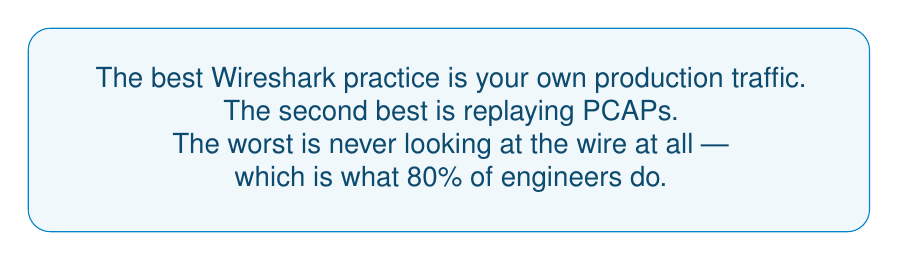
\begin{tikzpicture}
  \node[draw=wsblue, rounded corners=8pt, inner sep=14pt, fill=wsblue!6]{
    \parbox{0.8\textwidth}{\centering\sffamily\color{wsnavy}
      The best Wireshark practice is your own production traffic.\\
      The second best is replaying PCAPs.\\
      The worst is never looking at the wire at all ---\\
      which is what 80\% of engineers do.
    }
  };
\end{tikzpicture}
\end{center}

\end{document}
